\graphicspath{{results/fig/}}

\chapter{Results}
\label{chap:results}
An incremental approach to testing was done for this project. Each software component was tested individually. This section will report on the results of the incremental testing as well as the results of the entire system. As a sanity check, the results will also be compared to the results in \cite{fluxNoiseSquidsStevenAnton}. Lastly the entire system will be used to calculate the flux noise power of a real SQUID design. The results will be compared to the measured noise power for each design. 
\section{The noise extraction module}
The accuracy of this module is tested by comparing its output to a numerical solution for the given geometry. This module is tested without mesh optimisation. It is tested before the mesh optimisation module because the test setup for the mesh optimisation module requires the use of the noise extraction module.
\subsection{Test setup}
The aim of this project is not to verify the numerical framework proposed in \cite{fluxNoiseSquidsStevenAnton}. The testing should reflect this. As such the test setup is designed to verify the functionality of the implementation allowing the geometry of such a setup to not be limited by realistic designs for SQUID washers. Equation \ref{eq:MSFNfinal} describes the analytical solution for a thin wire loop. The assumption made in the derivation of this equation is that $R >> D$. The test is performed was a parameter sweep from $R = \si{8}{\mu m}$ and $D = \si{5}{\mu m}$ to $R = \si{45}{\mu m}$ and $D = \si{0.4}{\mu m}$ as shown figure \ref{fig:meshedTorus}. The parameter sweep was automated using a python script.

\begin{figure}[h]
    \centering
    \begin{subfigure}[b]{0.45\textwidth}
        \centering
        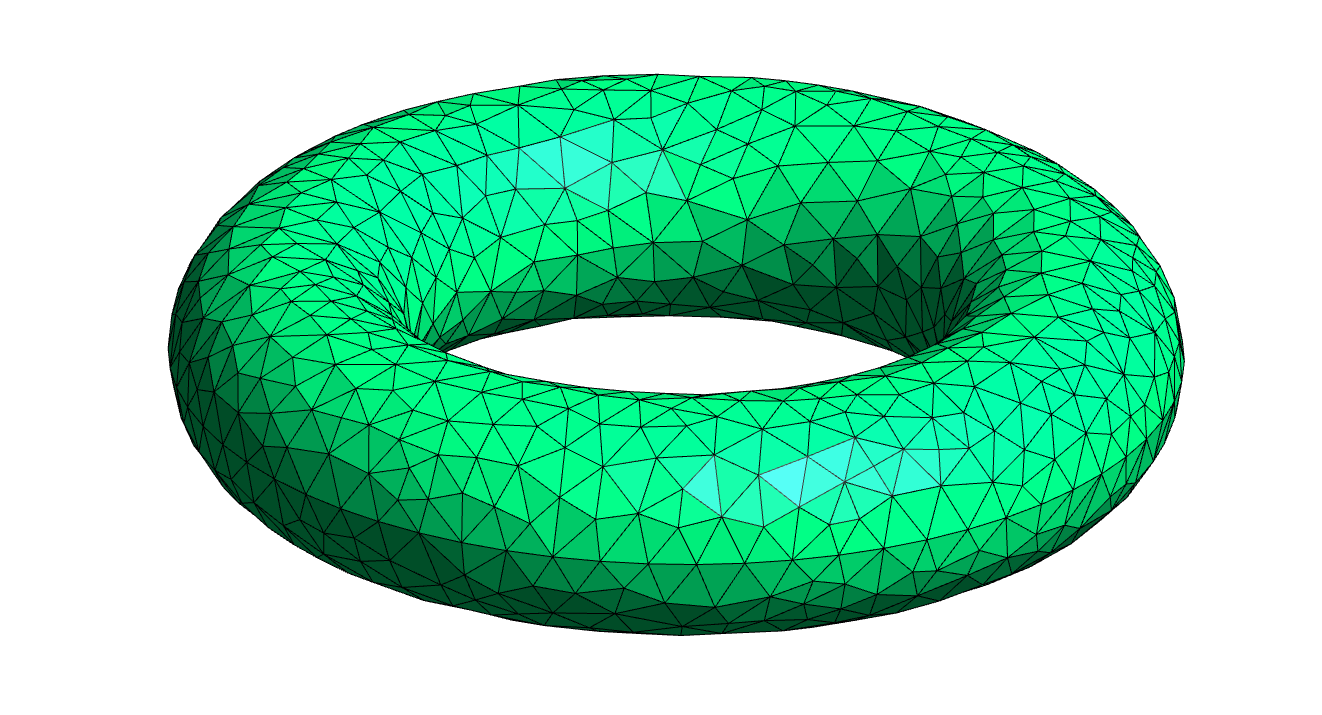
\includegraphics[width=0.5\textwidth]{torusThick}
        \caption{The meshed torus with the smallest loop radius and largest wire diameter}
    \end{subfigure}
    \hfill
    \begin{subfigure}[b]{0.45\textwidth}
        \centering
        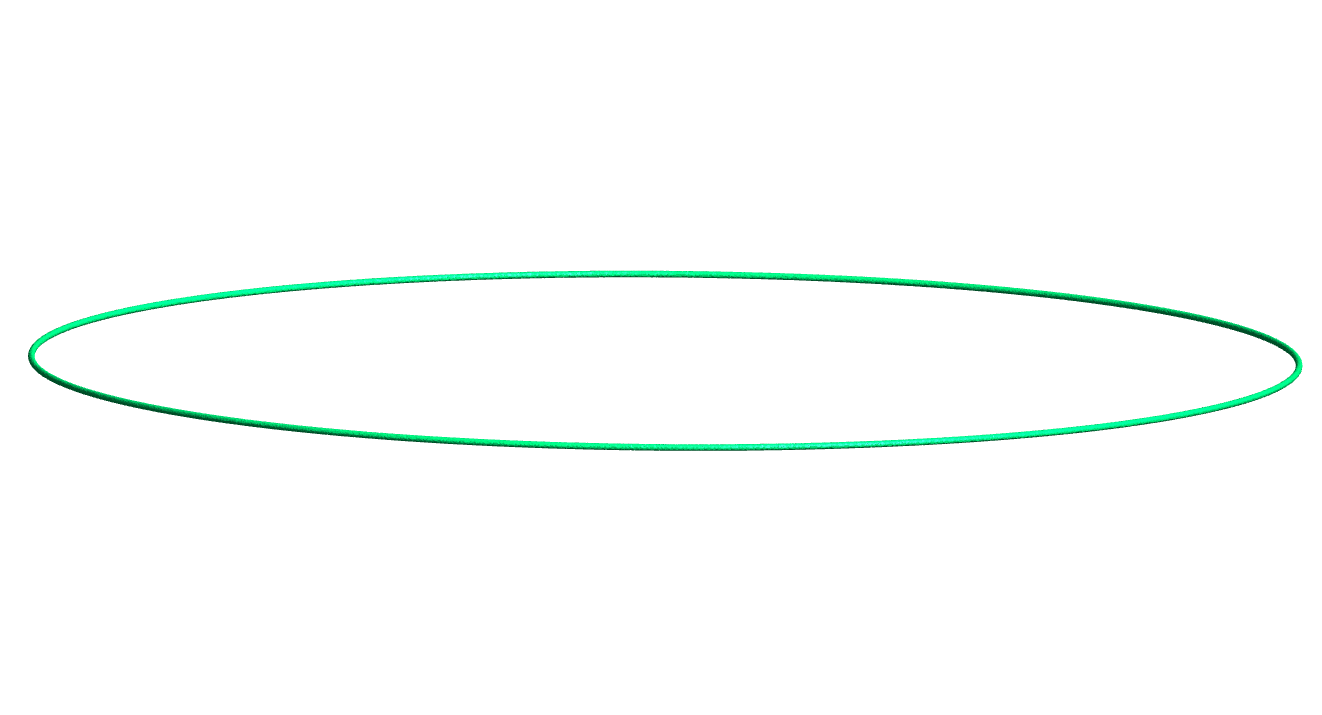
\includegraphics[width=0.5\textwidth]{torusThin}
        \caption{The meshed torus with the largest loop radius and smallest wire diameter}
    \end{subfigure}
    \caption{A figure showing the two extremes of the parameter sweep for a torus. The images show the surface mesh as generated by GMSH.}
    \label{fig:meshedTorus}
\end{figure}
\subsection{Results}

The results of the parameter sweep are summarized in figure \ref{fig:resTorus}.
\begin{figure}[H]
    \centering
    \begin{subfigure}[b]{0.48\textwidth}
        \centering
        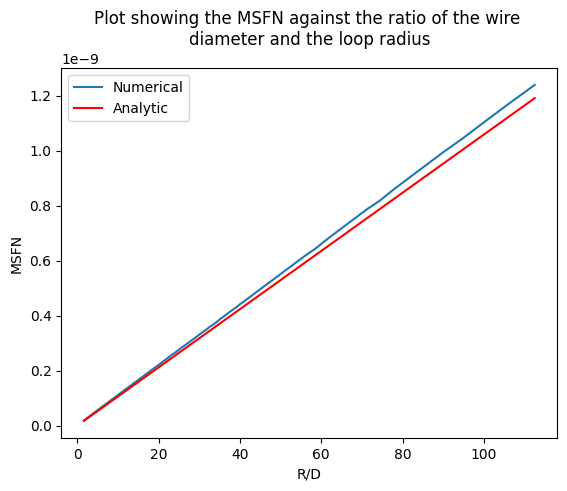
\includegraphics[width=\textwidth]{torusAVN}
        \caption{The analytical and numerical solutions for the parameter sweep}
        \label{fig:MSFNvRD}
    \end{subfigure}
    \hfill
    \begin{subfigure}[b]{0.48\textwidth}
        \centering
        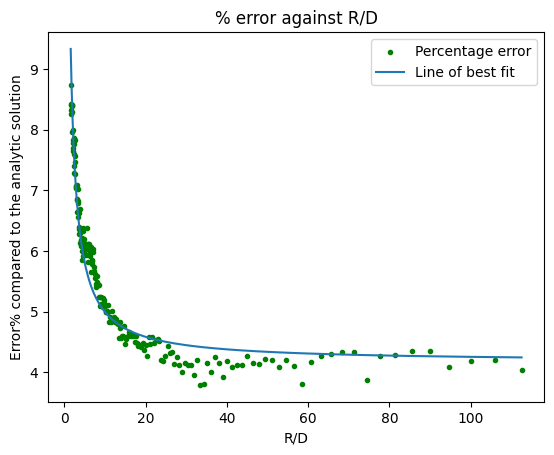
\includegraphics[width=\textwidth]{torusEVRD}
        \caption{The error plotted against the $R/D$}
        \label{fig:evRD}
    \end{subfigure}
    \caption{The figure shows both the MSFN ($\Phi_0^2 / Hz$) and the error compared to the analytic solution for the parameter sweep.}
    \label{fig:resTorus}
\end{figure}
From figure \ref{fig:resTorus} it is clear to see that the relative percentage error compared to the analytic solution decreases as the ration of the loop radius to diameter increases. This behaviour can be attributed to the assumption: $R >> D$. The decrease in error clearly demonstrates that the noise extraction module works for this particular setup. In figure \ref{fig:MSFNvRD} the analytical and numerical results increase linearly with an increase in $\frac{R}{D}$ as expected.

\section{The mesh optimisation module}
The geometry used to test the noise extraction module is not ideal for testing the mesh optimisation algorithm. To understand why this is the case, one must consider the assumption made to derive the analytic solution. By assuming that $R >> D$ you can approximate the ring as an infinitely long wire. By extension this assumes that the magnetic flux density and current density is uniform across the surface of the ring. The testing of the noise extraction module showed that the approximation is quite good. As a consequence, the mesh optimisation algorithm does not do much because the consistent current distribution leads to the mesh being over refined everywhere or not refined at all.
\subsection{Test setup}
To test this module a thin film circular ring of loop radius $R$ and track width $W$ is used. Essentially 3 questions must be answered. How many optimisation iterations is required, how much faster the problem is solved with the optimized mesh and if the subsequent extra executions of GMSH and TetraHenry needed to optimize the mesh is worth the trouble. \par
The test setup once again consists of a parameter sweep of $R$ and $W$ over the ranges $10 \mu m \le R \le 15 \mu m $ and $  3 \mu m \le W \le7\mu m$. The two extremes of the parameter sweep is shown in figure \ref{fig:testloop}. Simulations are run at 10 linearly spaced points in these intervals. For each simulation iteration, 4 mesh optimisation iterations are run. The initial characteristic length is determined by GMSH. The average mesh element count was $1500$ elements. Testing is once again completely automated with python. At each iteration the script records a number of statistics. The script records the execution times of TetraHenry and GMSH. It keeps track of both the simulation iteration and the mesh optimisation iteration. The results are written to a CSV file to be analysed with the \textit{"pandas"} python package. 
\begin{figure}[H]
    \centering
    \begin{subfigure}[b]{0.48\textwidth}
        \centering
        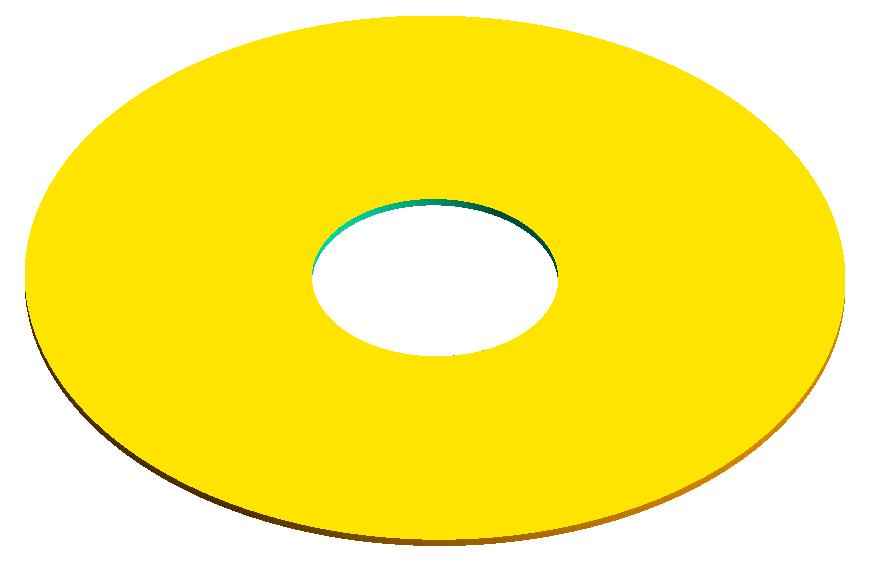
\includegraphics[width=\textwidth]{thickloop}
        \caption{The geometry of the test setup for the first iteration}
        \label{fig:thickloop}
    \end{subfigure}
    \hfill
    \begin{subfigure}[b]{0.48\textwidth}
        \centering
        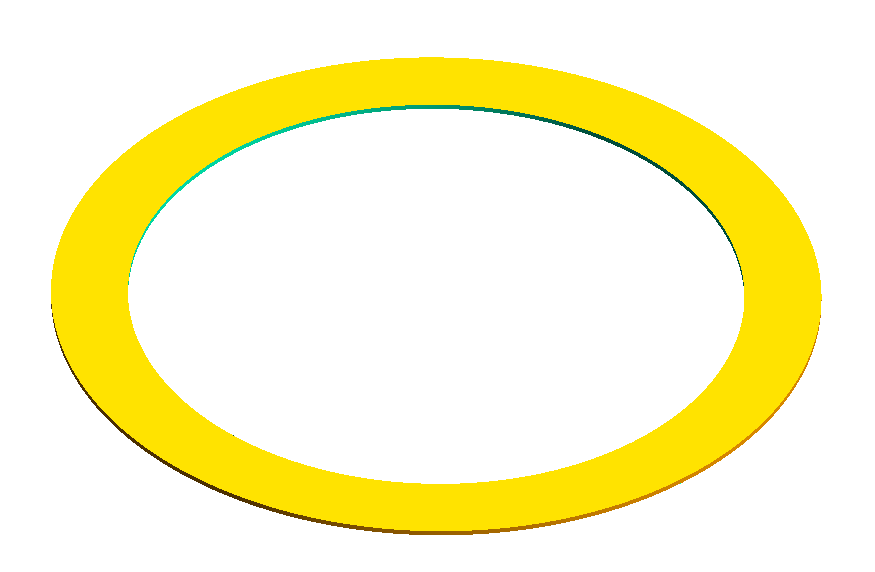
\includegraphics[width=\textwidth]{thinloop}
        \caption{The geometry of the test setup for the last iteration}
        \label{fig:thinloop}
    \end{subfigure}
    \caption{The figure shows the 2 extremes in the parameter sweep for the thin film circular loop experiment. The track thickness is set to $0.1 \mu m$}
    \label{fig:testloop}
\end{figure}
To assess the effectivity of the mesh optimisation algorithm it is necessary to make a baseline measurement. The baseline is set by forcing a minimum characteristic length in the optimized mesh and comparing the result to an unoptimized mesh with characteristic length equal to the minimum characteristic length in the optimized mesh. \par

The baseline simulations require significant computing resources and will run on a different system to the simulations with mesh optimisation enabled.
The total runtime of the baseline will be estimated. This is done by fitting a second order polynomial to the trend between the simulation time and number of nodes in the mesh. It was found through experimentation that for the specific geometry in question, the simulation time is roughly proportional to the square of the number of nodes in the mesh motivating the choice of a second order polynomial. This is necessary because simply comparing the number of nodes in both the optimized and unoptimized does not give a good indication of the difference in computational effort to solve either problems. The use of time as a metric accounts for the approximate quadratic relationship between the number nodes and the computational effort.

\subsection{Results}

To determine the number of optimisation steps necessary for convergence, the average relative error between the mean square flux noise figure calculated at each optimisation iteration and the value obtained after the $4_{th}$ optimisation iteration is calculated. The result is summarized in table \ref{tab:relerr}.


\begin{table}[H]
    \centering
    \begin{tabular}{lll}
    \hline
    Iteration number & Relative percentage error & Change in relative error \\ \hline
    0                & 1.520356                  & N/A                      \\
    1                & 0.47945                   & 1.040906                 \\
    2                & 0.028596                  & 0.450854                 \\
    3                & 0.001191                  & 0.027405                 \\
    4                & 0.000065                  & 0.001126                 \\ \hline         
    \end{tabular}
    \caption{Table of relative errors for each mesh optimisation cycle}
    \label{tab:relerr}
\end{table}

Table \ref{tab:relerr} gives some indication that after 4 iterations the solution becomes relatively stable. If we accept the 4 mesh optimisation iteration as being the correct result we can normalise the relative error and plot it against the normalised, cumulative time GMSH and TetraHenry took after each iteration. Figure \ref{fig:errvtime} shows this relationship.

\begin{figure}[H]
    \centering
    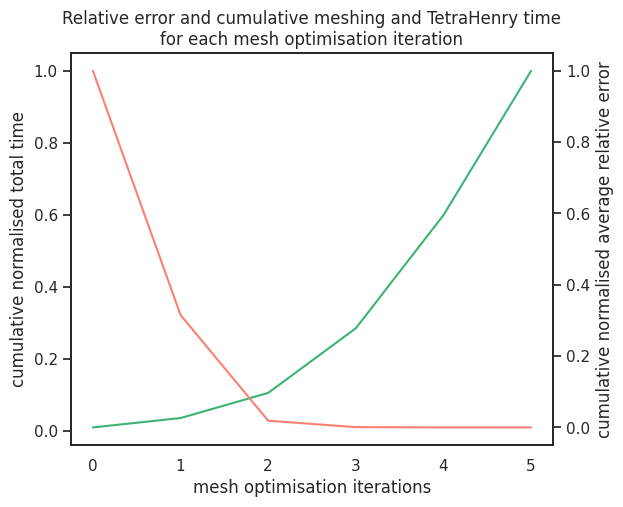
\includegraphics[width=0.5\linewidth]{errvtime}
    \caption{The figure shows the relative normalised error and the cumulative total time that GMSH and TetraHenry took at each optimisation step. The green line is the total time and the red line is the error.}
    \label{fig:errvtime}
\end{figure}

The optimal number of mesh iterations steps to minimize the time taken, and the error is between 1 and 2 iterations. The choice ultimately comes down to how accurate the user would like the solution to be. To compare the optimized mesh performance to the baseline, 2 will be selected as the optimal number of iterations.

\begin{figure}[H]
    \centering
    \begin{subfigure}[b]{0.48\textwidth}
        \centering
        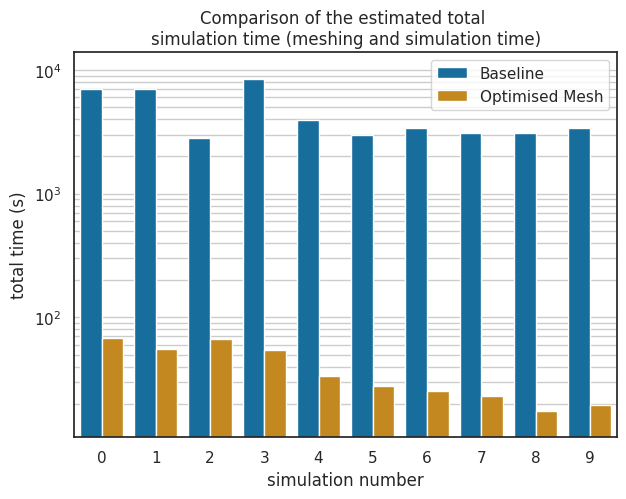
\includegraphics[width=\textwidth]{timevsimnum}
        \caption{The estimated time plotted for each simulation}
        \label{fig:timevssinnum}
    \end{subfigure}
    \hfill
    \begin{subfigure}[b]{0.48\textwidth}
        \centering
        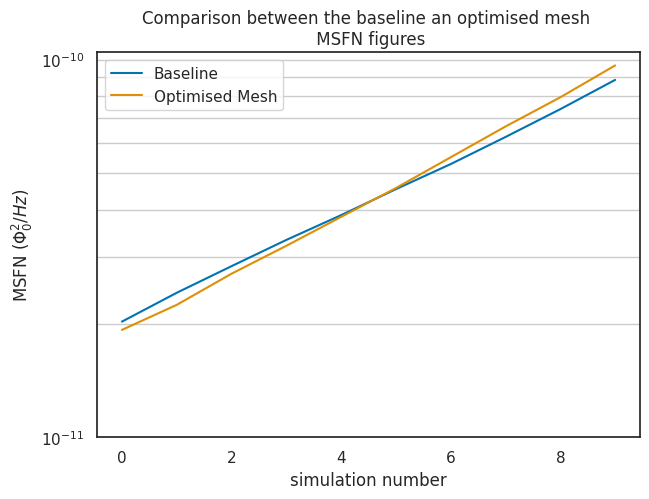
\includegraphics[width=\textwidth]{msfnvssimnum}
        \caption{The MSFN figure plotted for each simulation}
        \label{fig:msfnvssimnum}
    \end{subfigure}
    \caption{The figure shows the comparisons used to determine the accuracy and performance of the optimized mesh.}
    \label{fig:resCompOpt}
\end{figure}

Figure \ref{fig:timevssinnum} shows the estimated time to complete each simulation for the baseline as well as the optimized mesh. The result is plotted on a logarithmic scale. To estimate the time taken for the entire mesh optimisation process, the sum of the number of nodes in the mesh at each optimisation iteration is used. Figure \ref{fig:timevssinnum} shows the performance benefits of using the mesh optimisation module. On average, the computation time is decreased by a factor of 120. The best performance of the optimisation module decreased the computation time by a factor of 180 and the worst by a factor of 42. From this analysis it is clear that the mesh optimisation module provides major performance benefits. \par
Figure \ref{fig:msfnvssimnum} is used to determine the effect that optimisation has on the accuracy of the resulting MSFN figure. The relative error for each simulation is used to assess the accuracy. The average relative error was $4.86\%$. The minimum and maximum relative error was $0.66\%$ and $8.42\%$ respectively. Figure \ref{fig:msfnvssimnum} shows the optimized mesh follows the same trend as the baseline. A maximum error of $8.42\%$ is acceptable when the performance benefits of using the mesh optimisation module is considered.

\section{Comparison with the results of S.M. Anton \textit{et al.}}
\subsection{Test Setup}
To verify the implementation of the numerical framework, a comparison with the results in \cite{fluxNoiseSquidsStevenAnton} is made. The same test will run for the exact same geometry. The setup chosen for this project consists of a square washer with a fixed square hole with a width of $10 \mu m$. The line width is then swept from $0.5 \mu m$ to $10 \mu m$. Figure \ref{fig:sqwasher} shows the geometry in the test setup. The film thickness is $150 \mu m$ and the penetration depth is identical to that used in \cite{fluxNoiseSquidsStevenAnton} and is set to $90 nm$. The implementation used in \cite{fluxNoiseSquidsStevenAnton} can be found here \cite{msfnCode} 

\begin{figure}[H]
    \centering
    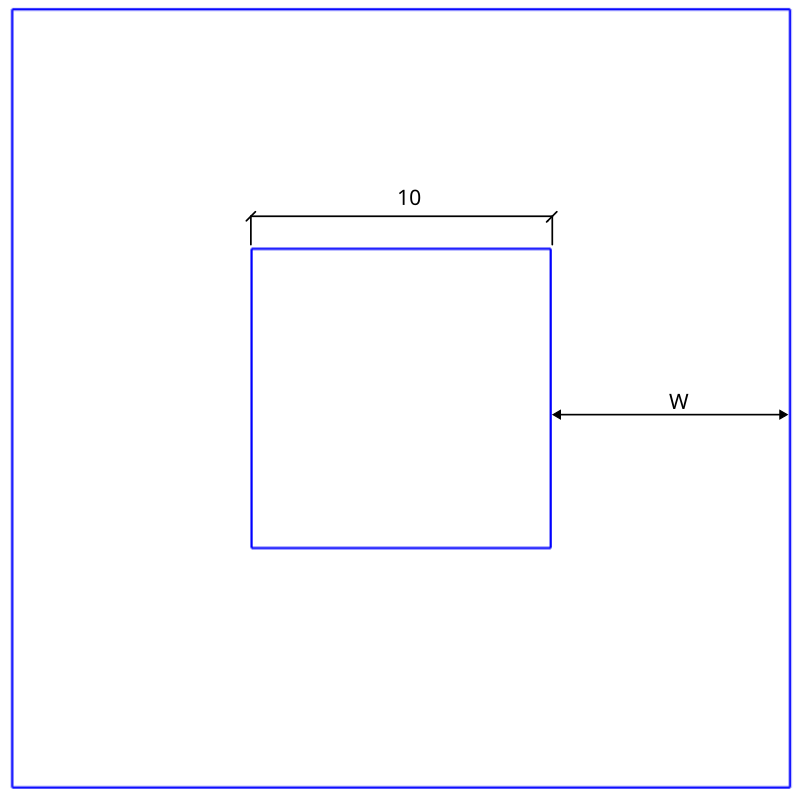
\includegraphics[width=0.3\linewidth]{sqwasher}
    \caption{The figure shows the geometry of the test washer in GMSH. All dimension are in $\mu m$}
    \label{fig:sqwasher}
\end{figure}

\subsection{Results}
Figure \ref{fig:steveComp} shows the results obtained by running the test setup. 
\begin{figure}[H]

    \centering
    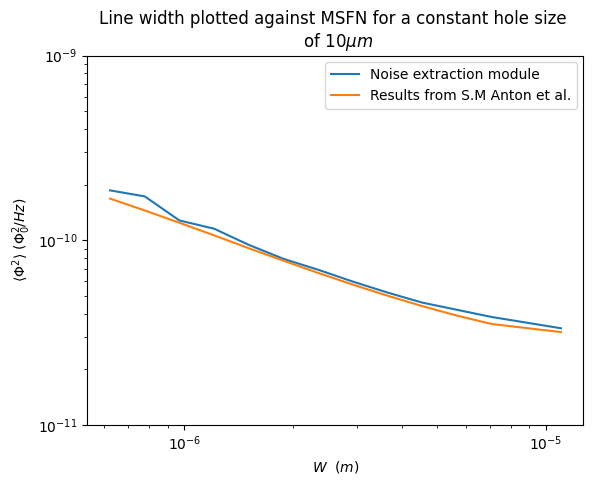
\includegraphics[width=0.4\linewidth]{steveComp}
    \caption{The plot shows the MSFN figure calculated by the noise extraction module as well as the figure calculated using \cite{msfnCode}}
    \label{fig:steveComp}
\end{figure}
From figure \ref{fig:steveComp} it is clear to see that the noise extraction module produces values in agreement with those obtained by S.M. Anton \textit{et al.} in \cite{fluxNoiseSquidsStevenAnton}. As shown in the previous section, the error decreases for an increase in optimisation iterations. One can therefore expect the noise extraction module to conform more closely to the results by S.M. Anton \textit{et al.} for a higher number of optimisation iterations. This could unfortunately not be tested due to memory limitations.

\section{Comparison with actual SQUID designs}
\subsection{Test setup}
The authors of \cite{fluxNoiseSquidsStevenAnton} performed accurate measurements of the PSD of a variety of SQUIDs. The authors also calculated the inferred MSFN by fitting each spectrum to equation \ref{eq:PSDfit}. Once the parameters in equation \ref{eq:PSDfit} where determined the authors calculated the MSFN figure. The authors measured MSFN values on 2 groups of SQUIDs. Both groups utilised Nb-AlOx-Nb junctions. The SQUIDs in group \textit{I} had film thickness of $150 nm$ and the SQUIDs in group \textit{II} had a film thickness of $200 nm$. 
\begin{equation}
    S_\Phi (f) = Af^{-\alpha}+C
    \label{eq:PSDfit}
\end{equation}
Both groups utilised the same square washer design but varied different parameters across each SQUID in the group. Group \textit{I} fixed the track width while varying the width of the washer. Group \textit{II} varied both the track width and the width of the washer. Table \ref{tab:sweepres} shows the results of the parameter sweep as well as the values of each parameter used in the sweep and figure \ref{fig:sqsweep} shows the square washer design along with what each parameter refers to.

\begin{figure}[H]
    \centering
    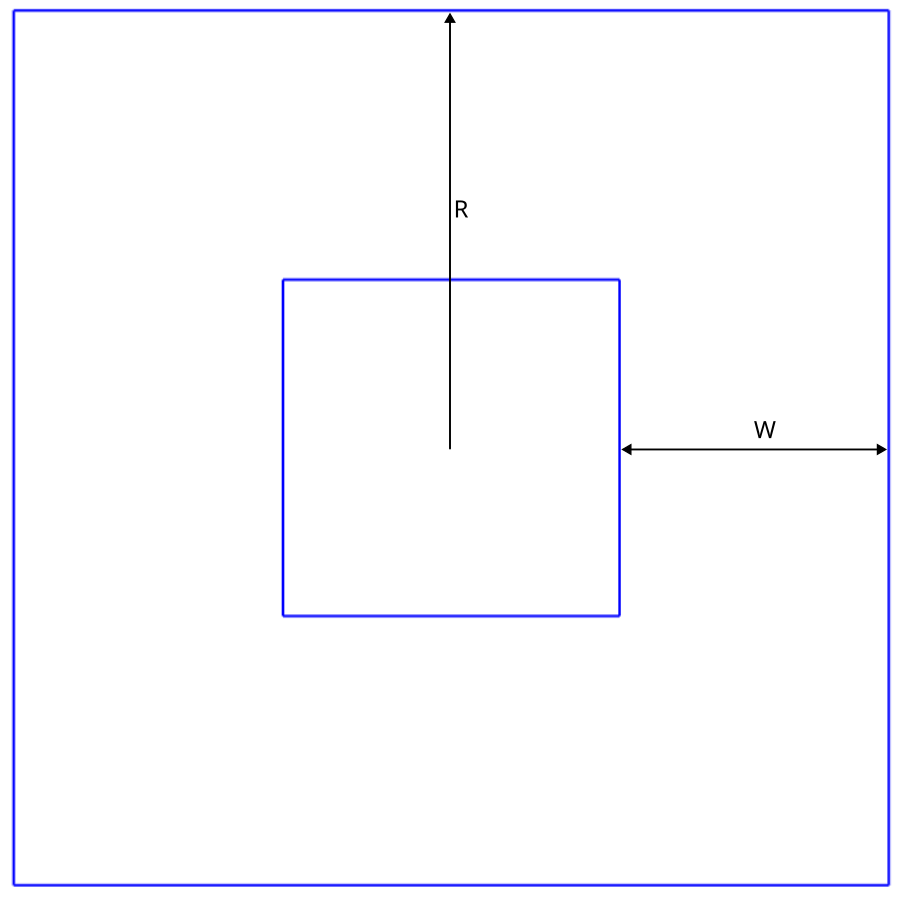
\includegraphics[width=0.4\linewidth]{sqsweep}
    \caption{A figure showing the parameters that are changed during the parameter sweep. W is referred to as the track width and R is referred to as the loop radius. 2R is the SQUID width.}
    \label{fig:sqsweep}
\end{figure}
\subsection{Results}
The MSFN figure cannot be measured directly. The power spectral density of the noise is measured. To relate the power spectral density to the mean square flux noise one can simply apply equation \ref{eq:PSDtoMSFN}.
\begin{equation}
    \langle \Phi^2 \rangle = \int_{f_1}^{f_2}S_\Phi (f) df
    \label{eq:PSDtoMSFN}
\end{equation} 
The limits of the integral are still the subject of debate \cite{fluxNoiseSquidsStevenAnton}. This is important to take note of as the choice of integration limits directly influence the result. The measured noise power in \cite{fluxNoiseSquidsStevenAnton} was calculated using $f_1 = 10^{-3}$ and $f_2 = 10^9$. Table \ref{tab:sweepres} shows the results of the parameter sweep. Figure \ref{fig:stevefig} is taken directly from \cite{fluxNoiseSquidsStevenAnton} and shows the flux noise measurements. For this comparison only the measurements at $0.1 K$ is used. 
\begin{table}[H]
    \centering   
    \begin{tabular}{lllll}
        \hline
        SQUID Number & R & W & MSFN (measured) ($\frac{\si{\nano}\Phi_0^2}{Hz}$) & MSFN (numerical) ($\frac{\si{\nano}\Phi_0^2}{Hz}$)\\ \hline
        I.1 & 12 & 0.5 & 4.5 & 111.924000 \\
        I.2 & 6 & 0.5 & 3 & 88.018600 \\
        I.3 & 3 & 0.5 & 1.2 & 0.121771 \\
        II.5 & 40 & 15 & 1 & 0.110498 \\
        II.1 & 265 & 240 & 2 & 0.098736 \\
        II.3 & 85 & 60 & 0.8 & 0.043155 \\ \hline
    \end{tabular}
    \caption{The table shows the measured MSFN figures from \cite{fluxNoiseSquidsStevenAnton} and the MSFN values calculated using the noise extraction module. The parameters R and W are listed in $\si{\micro m}$. The SQUID number uses the same numbering as used in \cite{fluxNoiseSquidsStevenAnton}. The table is sorted by the numerical MSFN figure in ascending order.}
    \label{tab:sweepres}
\end{table}

\begin{figure}[h]
    \centering
    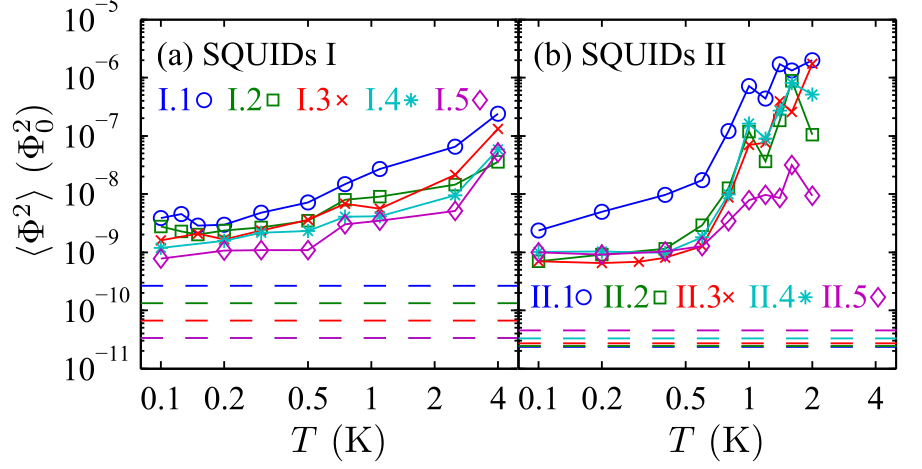
\includegraphics[width=0.5\linewidth]{stevenfig}
    \caption{The figure shows the various flux noise measurements taken in \cite{fluxNoiseSquidsStevenAnton}. The dashed line is predicted flux noise from the analytic equation \ref{eq:ThinFilmMSFN}.}
    \label{fig:stevefig}
\end{figure}

Table \ref{tab:sweepres} demonstrates that there is a large discrepancy between the measured MSFN figures and the figures calculated using the noise extraction module. If we only consider SQUIDs in group \textit{I} for the moment, we observe that the noise extraction module calculates MSFN figures that follow the same trend as the measured values. The SQUID with the largest measured MSFN value is also the SQUID with the largest MSFN figure calculated by the noise extraction module. If we consider only the SQUIDs in group \textit{II} then this trend is violated. We do note that in group 2 the analytical predictions roughly follow the same trend. The authors noted that a potential source of error in the inferred MSFN figures is the sensitivity of the alpha parameter. Fitting the measured PSD to equation \ref{eq:PSDfit} will lead to some error. The authors noted that at low temperatures a $0.03$ change in $\alpha$ can change the inferred MSFN figure by a factor of $1.6$. The violation of the trend in group \textit{II} can easily be accounted for by error in the $\alpha$ parameter. The authors also noted their difficulty in reconciling their data with the uncorrelated surface spin model and suggested that their data is consistent with a model where there is strong correlation between individual spins \cite{fluxNoiseSquidsStevenAnton}. \par
In this context one could make the argument that the module is useful for design as it can enable designers to compare designs but not useful for accurately predicting MSFN figures. More data over a wider range is required to conclusively make this claim as errors in fitting the data makes it hard to compare designs with similar MSFN figures.